\section{Цель}

Исследование характеристик дискретной марковской цепи и ее состояний.

\section{Порядок выполнения}

\begin{enumerate}
    \item Разработайте программу экспериментальных исследований дискретной марковской цепи с заданной матрицей переходных вероятностей G.
    \item Осуществите прогоны модели с начальными значениями, соответствующими состояниям дискретной марковской цепи.
    \item Выведите на экран диаграммы изменения состояния дискретной марковской цепи.
    \item Для каждого состояния дискретной марковской цепи определите его вид, определите классы эквивалентных состояний.
    \item Спланируйте и осуществите эксперименты для определения стационарного распределения вероятностей дискретной марковской цепи.
    \item Рассчитайте стационарное распределение вероятностей дискретной марковской цепи и сравните его с распределением, построенным по результатам экспериментов.
\end{enumerate}

\section{Исходные данные}

Матрица переходных состояний $G$.

\[
    G=
    \begin{vmatrix}
        0.3&0.3&0&0.4\\
        0.7&0.3&0&0\\
        0&0&0.4&0.6\\
        0&0&0.2&0.8\\
    \end{vmatrix}
\]

В качестве начальных значений линейного конгруентного генератора используются следующие величины:

$m=2^31 - 1$
$a=630360016$
$e_0=42352531$

\section{Прогоны модели}

Для отображения диаграмм изменения состояния дискретной марковской цепи были совершены $4$ прогона модели
с начальными состояниями равными каждому из состояний. При каждом прогоне было совершено $200$ переход между
состояниями.

\begin{figure}[h!]
    \centering
    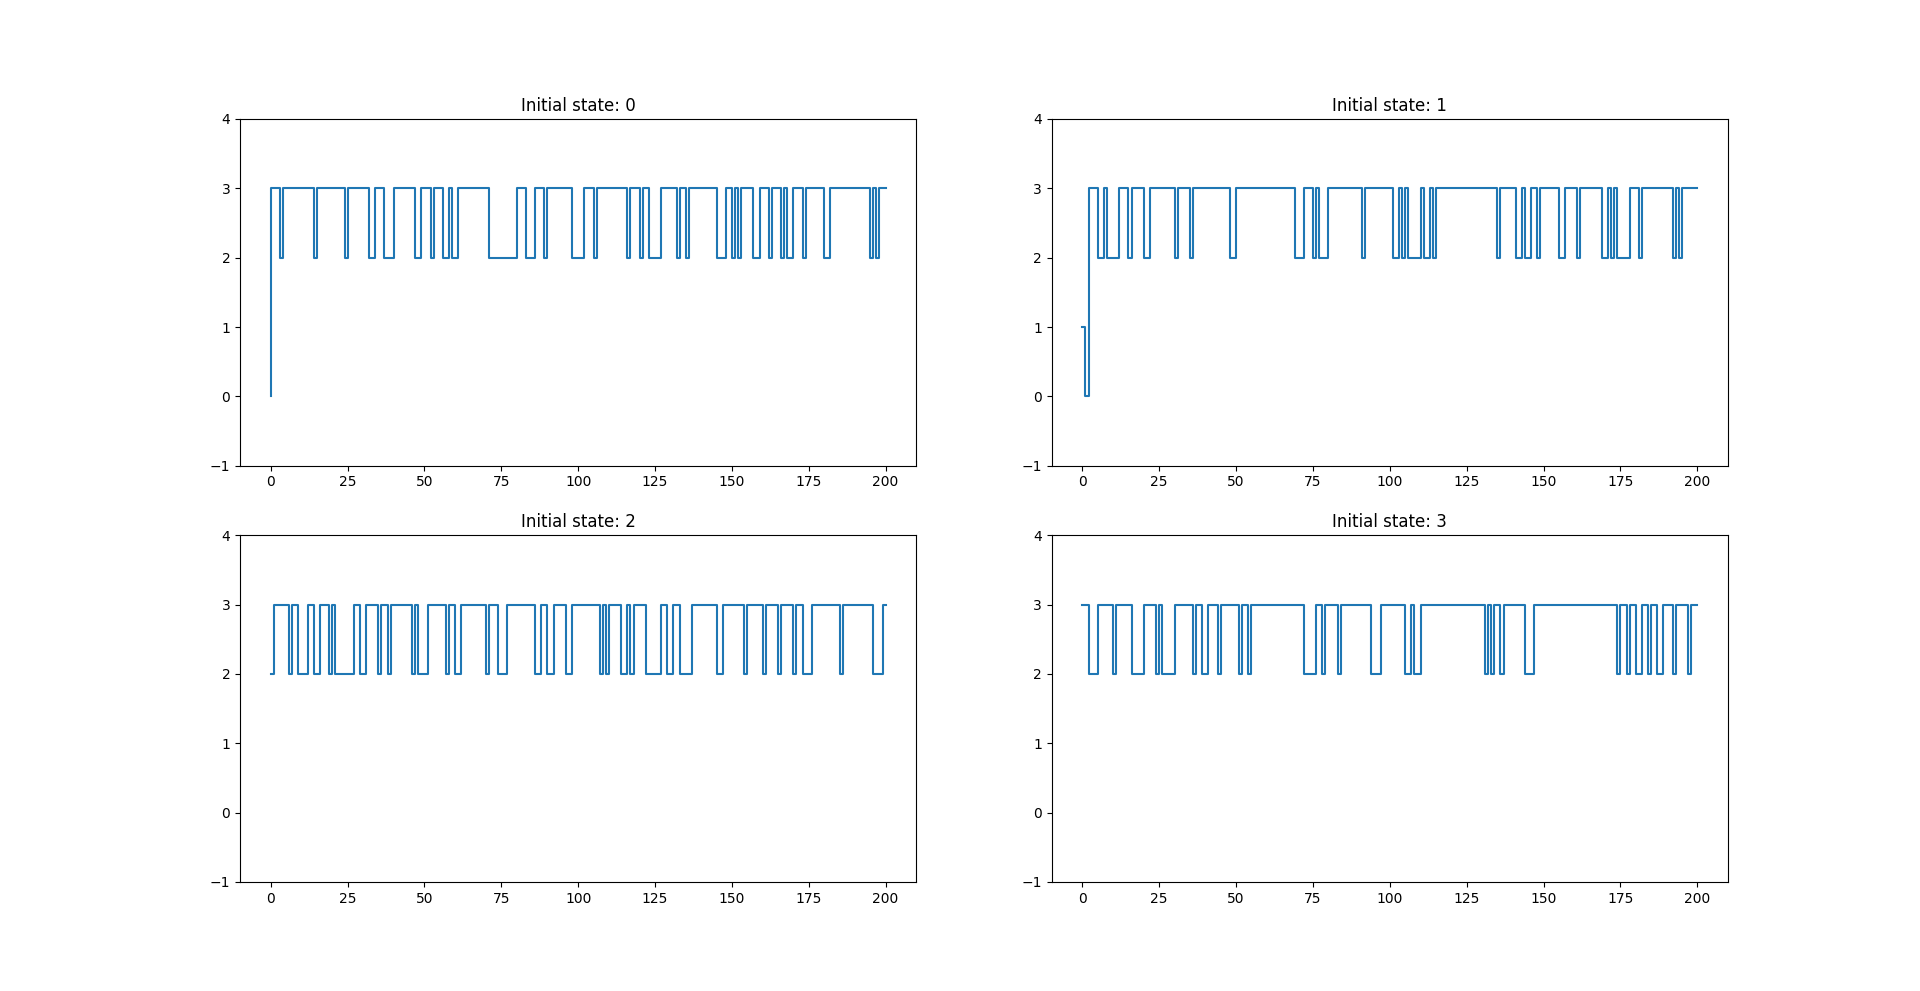
\includegraphics[width=\textwidth]{img/initial_runs.png}
    \caption{Прогоны модели с различными начальными состояниями}
\end{figure}

\section{Классификация состояний}

\textit{Состояние 1} - несущественное, нулевое, возвратное, непериодическое.
\textit{Состояние 2} - несущественное, нулевое, возвратное, непериодическое.
\textit{Состояние 3} - существенное, положительное, возвратное, непериодическое.
\textit{Состояние 4} - существенное, положительное, возвратное, непериодическое.

Состояния 3 и 4 являются сообщающимися состояниями.

\section{Стационарного распределение вероятностей}

\subsection{Экспериментальное распределене}

Для вычисления экспериментального распределения были выполнены $100$ прогонов моделей с различными начальными состояниями.
В результате были вычисленно стационарного распределение вероятностей, перечисленное ниже.

\[
  p1 = 0.00025\\
  p2 = 0.0003\\
  p3 = 0.25305\\
  p4 = 0.7464
\]

\subsection{Расчетное распределене}

Кроме того, было вычислено расчетное распределение вероятностей по формуле $p=pG$.

\[
  p1 = 0\\
  p2 = 0\\
  p3 = 0.25\\
  p4 = 0.75
\]

\section{Выводы}

В рамках выполнения настоящей лабораторной работы было проведено исследование дискретной марковской цепи и ее состояний.
Была выявлена группа сообщающихся состояний, а также определены свойства каждого из четырех состояний в отдельности.
Помимо прочего, полученные экспериментальные значения стационарного распределения вероятностей дискретной марковской цепи совпадают с
расчетными.

\section{Листинги}

\lstinputlisting[language=Python][caption=Листинг основного скрипта]{../lab.py}
\lstinputlisting[language=Python][caption=Листинг скрипта, содержащего модель дискретной марковской сети]{../markov.py}
\lstinputlisting[language=Python][caption=Листинг скрипта, содержащего линейный конгруентный генератор]{../../common/gen.py}
\lstinputlisting[language=Python][caption=Листинг скрипта, инициализируещего логирование]{../../common/log.py}
